\documentclass[12pt, dvipdfmx, default, cjk]{beamer}
\usetheme{Antibes}
\usecolortheme{beaver}
\usefonttheme{structurebold}
\setbeamertemplate{navigation symbols}{}
\setbeamertemplate{footline}[page, number]
%\useinnertheme{rectangles}
%\useoutertheme{smoothbars}

% \mathversion{bold}

\usepackage{graphicx}
\usepackage{amsmath, amssymb, cite, url}

%%%

\title{Weakly Supervision Twitter Profile}
\author{Speaker: @cympfh}
\date{\today}

\begin{document}

\begin{frame} \titlepage \end{frame}

\begin{frame}
  "Weakly Supervised User Profile Extraction from Twitter"
  Jiwei Li, Alan Ritter, Eduard Hovy, 2014

  を読みます.

  \vfill

  \begin{itemize}
    \item<2-> Twitter ユーザーの個人情報の推定
    \item<3-> 友達の推薦、広告とかに使える
    \item<4-> 実際、性別による広告ターゲティングが使われてる
      ("広告主の方へ:Twitterプロモ商品で性別のターゲティングが可能になりました")
    \item<5-> (個人的に) ネトストが効率化される
  \end{itemize}
\end{frame}

\begin{frame}{リンク}
\begin{itemize}
\item
  \url{http://aritter.github.io/}
  作者の一人のサイト
  \item
  \url{http://www.aclweb.org/anthology/P/P14/P14-1016.pdf}
  論文はここ
  \end{itemize}
\end{frame}

\begin{frame}{目次}
  \tableofcontents
\end{frame}

\section{導入}

\setbeamercovered{dynamic}
\begin{frame}
  ユーザーのツイートと
  友達関係から
  そのユーザーの
  (Facebookっぽい)
  プロフィールを
  生成する
  \begin{itemize}
    \item<1-2> 配偶者
    \item<1-2> 学歴 (在学してる大学)
    \item<1-2> 職業
    \item<-1> 趣味
    \item<-1> 宗教
    \item<-1> 出身地
    \item<-1> 現住所
    \item<-1> 家族
  \end{itemize}
\end{frame}

\begin{frame}
  ツイートの中で言及があれば、強い証拠になる.
  というか、そのような言及はあると仮定する.
  \begin{alertblock}{配偶者 (のTwitter ID)}
    @\alert {hogehoge} has taken all the kids today so I can go shopping - CHILD FREE!
  \end{alertblock}
  \begin{alertblock}{学歴 (学校の名前)}
    I got accepted to be part of the UofM engineering safety pilot program in \alert{FSU}.
  \end{alertblock}
  \begin{alertblock}{職業 (会社名)}
    first day of work at \alert{HuffPo}, a sports bar woo come visit me yo..
  \end{alertblock}
\end{frame}

\section{関連研究}

\begin{frame}{先行研究}
  \begin{itemize}
    \item Twitterのプロフィール当ての先行
      \begin{itemize}
        \item 年齢 -- Rao+ 2010
        \item 政治的意見(極性) -- Pennacchiotti \&Popescu 2011, Conovt+ 2011
        \item 性別 -- Ciot+ 2013, Liu \&Ruth 2013, Liu+2012
      \end{itemize}
    \item 訓練データの作成のコスト
      \begin{itemize}
        \item 例えば上の Cio+ 2013 は、プロフィール画像を人間が見て手で性別を書きだした
      \end{itemize}
  \end{itemize}
\end{frame}

\begin{frame}{知見}
  \begin{itemize}
    \item Distant supervision a.k.a. weak supervision
      \begin{itemize}
        \item 後述
      \end{itemize}
    \item Homophily
      \begin{itemize}
        \item (ネットにおける)友達関係は同じ属性 (趣味とか) を持ちやすい
        \item 今回の場合、「学歴」「職業」についてはかなり利きそう
        \item 逆に「配偶者」については全く効かなそう
        \item 属性の性質によって恣意的に
      \end{itemize}
  \end{itemize}
\end{frame}

\begin{frame}{Distant supervision}

  "Distant supervision for relation extraction without labeled data" \\
  Mintz+, 2009 \\
  \url{http://web.stanford.edu/~jurafsky/mintz.pdf}

  \vfill

  訓練データの作成に手でラベルを付与する代わりに、
  知識データベース (e.g. Freebase \footnote[frame]{\url{http://www.freebase.com/}})
  を間に挟んで手間を省く.

\end{frame}

\section{データ}

\begin{frame}{訓練データの作成}
  3つの属性
  
  \begin{itemize}
    \item 学歴
    \item 職業
    \item 配偶者
  \end{itemize}
  
  について、それぞれ、Twitter ID をノードとするグラフを3つ作る.
  (一つのユーザーについて3つの属性を揃えるわけではない)
\end{frame}

\begin{frame}
\begin{columns}
 \begin{column}{0.5\textwidth}
   学歴、職業、については
   Google+ を用いる.

   最終的にTwitter ID と紐付けしたいので、
   \begin{itemize}
     \item (「学歴」or
     \item「職業」) and
     \item「Twitterへのリンク」
   \end{itemize}
   を満たすプロフィールページを探す.

 \end{column}
 \begin{column}{0.5\textwidth}
   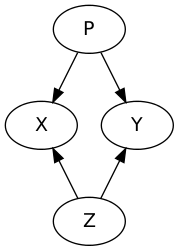
\includegraphics[width=1.0\textwidth,bb=0 0 935 571]{0.png}

   Google+ "knowledge base"
 \end{column}
 \end{columns}
\end{frame}

\begin{frame}{エイリアス}
  \begin{columns}
    \begin{column}{0.5\textwidth}
      データベースである Freebase を用いる

      \vfill

      "Harvard University"
      "Harvard"
      "Harvard U"

      $\rightarrow$ 何か一つ
    \end{column}
    \begin{column}{0.5\textwidth}
      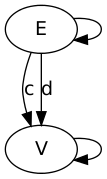
\includegraphics[width=1.0\textwidth,bb=0 0 376 325]{1.png}
    \end{column}
  \end{columns}
\end{frame}

\begin{frame}{データの広げ方}
  Google+, Twitter の友達関係の両方を用いて、
  ユーザーを追加してく.

  ただし、Twitter の友達関係は、あとで素性として使う.
\end{frame}

\begin{frame}[fragile]{配偶関係}
  \begin{columns}
    \begin{column}{0.5\textwidth}
      配偶者をわざわざ書かせるSNSはFacebookくらいしかないので、
      これを用いる. \\

      ただしこれだけだと少ないので
      Freebase
      を用いて
      \verb+/PEOPLE/PERSON/SPOUSE+
      にあるものを追加する.
    \end{column}
    \begin{column}{0.5\textwidth}
      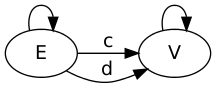
\includegraphics[width=1.0\textwidth,bb=0 0 582 562]{2.png}
    \end{column}
  \end{columns}
  \url{http://www.freebase.com/people/marriage?instances=}
\end{frame}

\def\isSpouseOf{\textrm{ isSpouseOf }}

\begin{frame}
  また配偶関係は反射関係を持つはず

  \[ a \isSpouseOf b = b \isSpouseOf a \]

  ことから, \\
  $a \isSpouseOf b$ かどうかが分からなくても、 \\
  $b \isSpouseOf a$ が分かれば、そちらも決定できる.

\end{frame}

\begin{frame}{データの統計}

  以上のように集めたデータセットを正のデータとする.
  異なる組み合わせを負のデータとして作る.

  \begin{tabular}{|l | c | c | c |} \hline
    & Education & Job & Spouse \\ \hline
    \#Users & 7,208 & 1,806 & 1,636  \\ \hline
    \#Pos Entities & 451 & 380 & 3121 \\ \hline
    \#Neg Entities & 7.0e6 & 4.4e6 & 8.8e6 \\ \hline
  \end{tabular}
  \\
  Table 2 の一部
\end{frame}

\section{モデル}

\begin{frame}
  提案されるモデル
\end{frame}

\def\zkie{z^k_{i,e}}
\def\zkix{z^k_{i,x}}

\begin{frame}{変数}

  \begin{itemize}
    \item ユーザー: $1 \le i, j \le M$
    \item 属性: $k = $ Spouse, Education, Job
    \item ユーザー$i$ によるツイート(集合): $X_i = \{x_{i,j}\}$
    \item エンティティ: $e$ (属性問わず)
    \item ユーザー$i$ の属性$k$ についての友達の集合: $F_i^k$
      \begin{itemize}
        \item $k =$ Education, Job の場合は単なるフォロー関係
        \item $k =$ Spouse の場合は、配偶者 の単集合
      \end{itemize}
    \item $\zkie$: ユーザー$i$の属性$k$が$e$であるかどうか
    \item $\zkix$: ユーザー$i$のツイート$x$が属性$k$についての言及であるかどうか
  \end{itemize}
\end{frame}

\begin{frame}{戦略}
  \begin{columns}
    \begin{column}{0.1\textwidth}
    \end{column}
    \begin{column}{0.9\textwidth}
      \begin{itemize}
        \item[GLOBAL] $\zkie$: ユーザー$i$の属性$k$が$e$であるかどうか
        \item[LOCAL] $\zkix$: ユーザー$i$のツイート$x$が属性$k$についての言及であるかどうか
      \end{itemize}

      最終的には $\zkie$ を知りたい.

      \alert{GLOBAL} は直接それを推定する.

      \alert{LOCAL} はツイートの単位で $\zkix$ を推定する.最後にORをとれば、

      \[ \zkie = \exists x \in \{ x | x \in X_i \land e \in x \} .~ \zkix \]

    \end{column}
  \end{columns}
\end{frame}

\begin{frame}{モデル}
  友達が $F^k_i$ で
  今までに $X_i$ という発言をしてきた
  ユーザー $i$
  の属性$k$ が $e$ である確率.

  \begin{alertblock}{Eq. 2}
  \[
    \Psi(\zkie, X_i, F^k_i  :  \Theta)
    \propto
    \Psi_{text}(\zkie, X_i) \times
    \Psi_{Neigh}(\zkie, F^k_i)
  \]
  \end{alertblock}

  右辺は、
  "テキスト的要因"
  と
  "隣人的要因"
  とに分離して独立と仮定している.

\end{frame}

\begin{frame}{テキスト的要因}
  エンティティ $e$ と テキスト $X_i$ から得る素性ベクトル
  を
  $\psi_{text}(\zkie, X_i)$
  として、

  \[
    \Psi_{text}(\zkie, X_i) = \exp \left[
      \Theta_{text}^k {}^T \cdot
      \psi_{text}(\zkie, X_i)
    \right]
  \]

  $\Theta_{text}^k$ は重みベクトル
\end{frame}

\begin{frame}{隣人的要因}
  ユーザー$i$の友達$j$の発言$X_j$を見て、決める.

  \[
    \Psi_{Neigh}(\zkie, F^k_i) = \prod_{j \in F_i^k} \Phi_{Neigh}(\zkie, X_j)
  \]

  where

  \[
    \Phi_{Neigh}(\zkie, X_j) = \exp \left[
      \Theta_{Neigh}^k {}^T \cdot
      \psi_{Neigh}(\zkie, X_j)
    \right]
  \]
\end{frame}

\begin{frame}{素性ベクトルの作り方}
  そんなに面白くない

  \begin{itemize}
    \item エンティティが大文字で始まるか
    \item エンティティの長さ
    \item POS tag
    \item \alert{エンティティの辞書にマッチする語がツイート中にあるかどうか}
  \end{itemize}
\end{frame}

\begin{frame}{配偶関係の場合の隣人関係}
  本来、ユーザー$i$の配偶者が$j$なら
  \[ F_i^{Spouse} = \{ j \} \]
  だけど、分からない間はそうはいかないので、
  ツイート中に現れたTwitter ID 全ての集合を用いる.
\end{frame}

\subsection{推定}

\begin{frame}[fragile]{推定のアルゴリズム}

  推定したいユーザーの周り ($F^k_i$) の属性が既知の場合と分かってない場合.

  現実世界においては、部分的には既知であることがある.

  \begin{itemize}
    \item NEIGH-OBSERVED
    \item NEIGH-LATENT
  \end{itemize}
\end{frame}

\begin{frame}{NEIGH-OBSERVED}
  周りの属性が既知なら、いきなり右辺が求まる.
          \[
            \zkie \leftarrow \textrm{argmax}_z \Psi(z, X_i, F^k_i)
          \]
\end{frame}

\begin{frame}[fragile]{NEIGHT-LATENT}
  \begin{columns}
    \begin{column}{0.4\textwidth}
      \begin{enumerate}
        \item[入力] $\{ (i, X_i, F^k_i) \}$
        \item[初期化] 全ての $\zkie$ を $\Psi_{text}$ で推定
        \item[更新] 収束するまで \verb+for-each i, e+
          \begin{itemize}
            \item $\zkie$ を $\Psi$ で推定
          \end{itemize}
          \[
            \zkie \leftarrow \textrm{argmax}_z \Psi(z, X_i, F^k_i)
          \]
      \end{enumerate}
    \end{column}
    \begin{column}{0.5\textwidth}
      \begin{alertblock}{Eq. 2 (再掲)}
        $\Psi(\zkie, X_i, F^k_i  :  \Theta)
          \propto
          \Psi_{text}(\zkie, X_i) \times
          \Psi_{Neigh}(\zkie, F^k_i)$
      \end{alertblock}
    \end{column}
  \end{columns}
\end{frame}

\section{実験}

\begin{frame}{ベースライン}
  \begin{columns}
    \begin{column}{0.1\textwidth}
    \end{column}
    \begin{column}{0.9\textwidth}
      \begin{itemize}
        \item [Only-text] さっきので $\Psi_{text}$ しか使わない
        \item [NELL] NELL\footnote{\url{http://rtw.ml.cmu.edu/rtw/kbbrowser/}}にある大学名と会社名のリストとマッチしたら true と答える \\ $\zkix$を当てる
      \end{itemize}
    \end{column}
  \end{columns}
\end{frame}

\begin{frame}{LOCALの実験}
  \begin{itemize}
    \item LOCAL(ENTITY): Entity-level: $\zkie$ を当てるタスク (GLOBALと同じ)
    \item LOCAL(TWEET): Tweet-level: $\zkix$ を当てる(サブ)タスク
  \end{itemize}
\end{frame}

\begin{frame}{結果}
  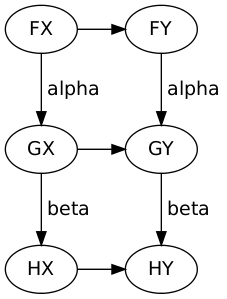
\includegraphics[width=1.0\textwidth,bb=0 0 1207 257]{3.png}
  精度は GLOBAL $>$ LOCAL \\
  再現は GLOBAL $<$ LOCAL --- LOCALにおいて$\zkie$は$\zkix$のORだから
\end{frame}

\begin{frame}
  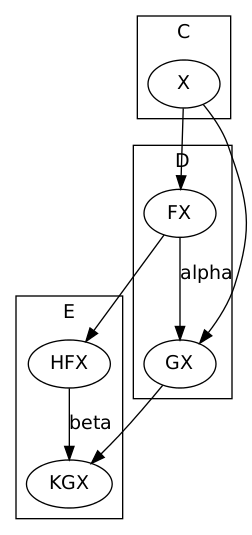
\includegraphics[width=1.0\textwidth,bb=0 0 1218 235]{4.png}
  \begin{itemize}
    \item 「学歴」より難しい (学生はすぐ宿題の話をするので簡単)
    \item Only-Text $<$ NEIGH-LATENT $<$ NEIGH-OBSERVED から、隣人関係の有用性が言える
  \end{itemize}
\end{frame}

\begin{frame}
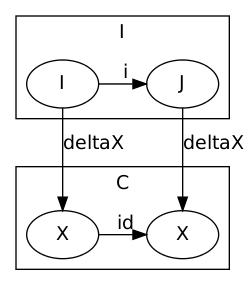
\includegraphics[width=1.0\textwidth,bb=0 0 1036 188]{5.png}
\end{frame}

\begin{frame}{まとめ、感想}
  \begin{itemize}
    \item 訓練データの作成には、属性ごとに工夫が必要
    \item 結果はそこまで属性によって偏らない
  \end{itemize}
\end{frame}

\end{document}
